\documentclass{article}
\usepackage[utf8]{inputenc}
\usepackage{mathtools}
\usepackage{amsmath}
\usepackage{amssymb}
\usepackage{witharrows}
\usepackage{cancel}
\newcommand{\norm}[1]{\left\lVert#1\right\rVert}
\newtheorem{definition}{Definition}[section]
\newtheorem{remark}{Remark}[section]
\newtheorem{theorem}{Theorem}[section]


\title{Deep Learning}
\author{Pietro Marcatti}
\date{First Semester 2022/2023}

\begin{document}

\maketitle
\section{History of Deep Learning}
\subsection{Perceptron}
The perceptron algorithm was invented in 1958. The perceptron became the first model for binary classification. It has one weight $w_i$ per input $x_i$. If the result is larger than a threshold it returns 1 otherwise 0 or -1 (non linearity ?).
To train a perceptron we repeat the following steps:
\begin{itemize}
    \item Initialize weigths randomly
    \item Take one sample $x_i$ and predict $y_i$
    \item For erroneous predictions update weights
    \begin{itemize}
        \item If prediction $y = 0$ and ground truth $y_i$ = 1, increase the weights
        \item If prediction $y = 1$ and ground truth $y_i$ = 0, decrease the weights
    \end{itemize}
    \item Repeat until no errors are made
\end{itemize}
However the perceptron can't solve a simple, although non-linear, problem such as the XOR. 
To improve on the perceptron model you must add new layers but there was a stagnation on the neural networks research. The stagnation was caused by a lack of motivation from the community due to the discouraging results of the first perceptron models. 
Still during the AI winter a couple important findings were published such as back-propagation and recurrent neural networks.\\\\
In 2009 the ImageNet dataset was published. It colleted images for each of the 100k terms in WordNet (16M images in total). Terms were organized hierearchally, es: Vehicle \textrightarrow Ambulance.
The ImageNet challange was instituted: 1 million images, 1000 classes, top-5 and top-1 error measured. To build ImageNet they started colleting candidate images from the internet. They then classified the candidates with Amazon Mechanical Turk service.\\
A more recent important achievement was the one obtained by AlphaGo a deep learning model, based on reinforced learning, that in 2016 defeated the best Go player.\\
Deep learning is the first class of learning algorithms that is scalable: performance just keeps getting better as you feed them more data. Instead when working on a small amount of data the performance of a traditional learning model (logistic regression, SVM, decision tree etc) is better.\\
The three key factors for deep learning scaling are:
\begin{itemize}
    \item Data
    \item Computation/hardware
    \item Algorithms
\end{itemize}

\section{Logistic Regression}
Let's start with a simple two feature model:
\begin{itemize}
    \item $x_1$ number of lectures you attend
    \item $x_2$ hours spent on the laboratory activities
\end{itemize}
With logistic regression we want to learn a probabilistic function:
$$\hat{y} = P(y=1|x)$$
In particular the goal is to find the parameters $w$ and $b$ of the following function (hypothesis).
$$H_{w,b}(x)= g =(w^T\cdot x+b) = \frac{1}{1+e^{-(w^T\cdot x+b)}}$$
where $g(z)$ is the sigmoid function so that:
$$\begin{cases}
    H_{w,b}(x) \geq 0.5 & \text{if } y=1\\
    H_{w,b}(x)<0.5 & \text{if } y=0
\end{cases}$$
To get our discrete classification we map the output of the hypthesis function as follow:
$$\begin{cases}
    H_{w,b}(x) \geq 0.5 & \text{\textrightarrow "1"}\\
    H_w,b(x)<0.5 & \text{\textrightarrow "0"}
\end{cases}$$
The decision boundary is $H_{w,b}(x) = 0.5 \rightarrow w^T\cdot x+b=0\rightarrow-3+x_1+2x_2$ supposing we have $b=3$ and $w=[1,2]$. The hypotesis function is $>0.5$ when the argument is $>0$, that is becuause of the shape and output of the sigmoid.

\subsection{Cost Function}
To find $w$ and $b$ so that:
$$\begin{cases}
    H_{w,b}(x) >= 0.5 & \text{if } y=1\\
    H_w,b(x)<0.5 & \text{if } y=0
\end{cases}$$
the logistic classifirer defines the following cost function:
\begin{equation}
    J(w,b) = \frac{1}{m}\cdot \sum_{i=1}^{m}{Cost(h_{w,b}(x^i),y^i)}
\end{equation}
\begin{equation}
    Cost(h_{w,b}(x^i),y^i)= -y^i\cdot ln(h_{w,b}(x^i))-(1-y^i)\cdot ln(1-h_{w,b}(x^i))
\end{equation}
This cost function or loss function is convex and is derivable respect to $w$ and $b$.
In general we call the function to learn the \textbf{hypotesis} but in deep learning it's also called \textbf{model}, while the \textbf{cost function} in deep learning is also called \textbf{loss function}.

\subsection{Gradient Descent}
Gradient descent is a general algorithm for minimizing derivable functions and we are applying it to linear regression.\\
The gradient descent algorithm repeats until convergence the following update on weigths:
\[ 
     \Theta_j = \Theta_j - \alpha \frac{\partial}{\partial\Theta_j}J(\vec{\Theta_0})
\]
It is always necessary to evaluate every new parameter before updating any of them as to not calculate the latters with the new values for the first ones.\\
The hyperparameter $\alpha$ is called the learning rate and it represents the size of the steps that we are taking down the direction of the gradient. For sufficiently small $\alpha$ the cost function should decrease on every iteration. This being said if $\alpha$ is too small it may take a big number of iteration to reach convergence. Finally, a value that is too big for $\alpha$ might cause the cost function to not decrease on every step because we might jump over the "dip", hence it might not converge. It is then a good idea to vary the parameter to experiment with the cost function and its convergence.
\subsubsection{Application of gradient descent on logistic regression}
Once we've established our decision function, in this example the logistic regression, we can procede to apply the gradient descent. To do that we first need to calculate the partial derivatives of the Loss function with respect to every parameter ($\vec{w}$ and $\vec{b}$) so that we can apply the changes. In this example with two inputs:
\begin{align*}
    w_1 &:= w_1 - \alpha \frac{\partial J(\vec{w},\vec{b})}{\partial w_1}\\
    w_2 &:= w_2 - \alpha \frac{\partial J(\vec{w},\vec{b})}{\partial w_2}\\
    b &:= b - \alpha \frac{\partial J(\vec{w},\vec{b})}{\partial b}\\
\end{align*}

\section{Neural Networks}
Neural Networks expand on the simple ideas of perceptron computing units by adding more layers on neurons betweeen the input and the output. As the shape of the neural network changes so does the way we represent it:
\begin{itemize}
    \item $W^{[j]}$: its the matrix of weights controlling the function mapping from layer j-1 to layer j
    \item $b^{[j]}$: the value of the bias for the j-th layer
    \item $a^{[j]}$: activation vector for the layer j
    \item $g^{[j]}$: activation function for the layer j
\end{itemize}
\subsection{Activation Functions}
In deep neural networks you also have to specify what activation function you want to apply to the activation vectors of each hidden layer. In the hidden layers we rarely see the sigmoid function because it is said to kill the gradient. This refers to the fact that the sigmoid, for particularly large or small inputs, saturates at 1 or 0 respectively. The hyperbolic tangent also suffers from this vanishing gradient problem but it generally performs better than the sigmoid. The sigmoid function is still widely used in the output or final layer to give a probabilistic meaning to our output as it's betweeen [0,1].\\
What are other types of activation function that we can be used in the hidden layers?
\begin{description}
    \item[ReLU or Rectified Linear Unit]:
        It's particularly easy to train and achieves great performance. Its derivative is particularly easy to calculate, given that you consider the point of non-derivability in 0. 
    \item[Leaky ReLU]: Leaky ReLU was created to solve the dying ReLU problem which affects neuron with ReLU activation functions. If their parameter is stuck at 0 no matter the input their output will be 0. If this happens no gradient flows and there cannot be any learning. To avoid this it assigns a slightly sloped straight line for the negative values.
\end{description}
It is fundamental to use non-linear activation functions otherwise the output of the neural network will be a simple linear combination of the inputs. Let's suppose our activation function is the identity function: $ g^{[1]}(z) = g^{[2]}(z) = z $ 
\[ 
    a^{[2]} = z^{[2]}= W^{[2]}a^{[2]}+b^{[2]} =  W^{[2]}(W^{[1]}x+b^{[1]})+b^{[2]} = (W^{[2]}W^{[1]})x + (W^{[2]}b^{[1]}+b^{[2]})
\]
We can define $ W' = W^{[2]}W^{[1]} $ and $ b'= W^{[2]}b^{[1]}+b^{[2]}$ then we can rewrite $ a^{[2]} = W'x +b'$. Linear activation function is then useless unless in the last layer when performing a regression task.
\subsection{Back propagation}
Back propagation is the concept and algorithm that allows to update the weights of the neural network to learn. It relies on two simple steps:
\begin{description}
    \item[Forward Step:] in this step is activated on one example and the error of each neuron of the output layer is computed.
    \item[Backwards Step:] in this step the network error is used for updating the weights. Starting at the output layer, the error is propagated backwards through the network layer by layer. This is done recursively computing the local gradient of each neuron.  
\end{description}
\begin{definition}[Jacobian Matrix]
    The derivative of a vector function (a vector whose components are functions) with respect to an input vector x is called a Jacobian Matrix and is represented as:
    \[ 
        \frac{\partial y}{\partial x}=
        \begin{bmatrix}
            \frac{\partial y_1}{\partial x_1} & \cdots & \frac{\partial y_1}{\partial x_n} \\
            \vdots & \ddots & \vdots \\
            \frac{\partial y_m}{\partial x_1} & \cdots & \frac{\partial y_m}{\partial x_n} \\
        \end{bmatrix}
    \]
    
\end{definition}
It is particularly important to set a reasonable initial value for the weights. If we used 0 on all weights, all $ z^{[1]} $ would be 0, hence $ a^{[1]}_1 = \ldots =a^{[1]}_n $ because we would always get the same mapping by the activation function. The derivaties used to obtain the gradient would be equal and so the weights and bias would all be changed by the same amount remaining all equal. We refer to this phenomenon as the symmetry problem and to counter it we can simply initialize the weights to a small random value. The reason for such a small value has to do with the previously mentioned vanishing problem. If your network starts working with big numbers it will get to the sigmoid in the output layer and be saturated on the 1 or 0 with very little gradient to move.

\subsection{Hyperparameters}
We've already referred to some of our variables as hyperparameters. We can identify an hyperparameter by considering if it is a variable that can be changed to impact the functioning and the performance of our model without it being a parameter such as the weights and the bias. Examples of hyperparameters are:
\begin{itemize}
    \item Learning rate
    \item Number of interaction (or epochs)
    \item Number of hidden layers
    \item Number of hidden units in each hidden layers
    \item Activation functions
\end{itemize}
The process of tuning these values to achieve the best result is for us, right now, all empirical.

\section{Improving our Neural Network}
In the process of training our neural network we often divide all the data we have available in two or three sets. These are the training and test set, plus optionally, the validation set. The training set contains the data we use to perform the learning of our model. If available we then measure the performance on the validation set in real world mock-up scenario. Eventually, when our model is stable we test it on the test set to get a real measure of it's performance.\\
It is fundamental that validation and test have the same distribution to ensure meaningful learning.\\
We divide our training data set into smaller batches of usually around 16-32-64 samples. We compute forward and backwards on every single sample. Once we complete all the batches we completed an epoch. We can then start again but now, on the first batch, our neural network will have weights that will have already changed thanks to all other batches.

\subsection{Overfit vs. Underfit}

\subsubsection{Regularization}
Logistic Regression: Minimization problem with regularization:$ \;\min_{w,b}{J(w,b)}$
$$J(w,b)= \frac{1}{m}\left[ \sum_{i=1}^{m}{Cost(h_{w,b}(x^{(i)}), y^{(i)})+\frac{\lambda}{2}\sum_{j=1}^{n}{w_i^2}} \right]$$
$\lambda$ is called the regularization parameter, usually b is ignored in the regularization process.
By setting a big regularization parameter we are saying that our minimization algorithm should focus on reducing the weights. The goal is to have the weights all in the same order of magnitude.\\\\
Doesn't regularization kill the importance of some features over others?\\\\
Regularization with Neural Networks:\\
$$J(W^{[1]}, b^{[1]}W^{[2]}, b^{[2]})= \frac{1}{m}\left[ \sum_{i=1}^{m}{\mathbb{L}(\hat{y}, y^{(i)})+\frac{\lambda}{2}\sum_{i=1}^{L}{\norm{W^{[l]}}^2_F}} \right]$$

Where $\lambda$ is the regularization parameter, l is the layer. $$\norm{W^{[i]}}^2_F=\sum_{i=1}^{n{[l-1]}}{\sum_{j=1}^{n^{[l]}}{(W_{i,j}^{[l]})^2}}$$
Where $W^{[l]}\in \mathbb{R}^{n^{[l]}\times n^{[l-1]}}$\\
Regularization helps preventing overfitting because by using a big value for $\lambda$ we minimize weigths close to 0 and some of them are basically dead (almost 0)\\\\
Too many dead nodes means underfitting? Would it ever be useful to have a small $\lambda$\\\\

\subsection*{Vanishing and Esploding Gradients}
We can observe this phenomenon when dealing with very deep neural networks. In summary, we want to initialize the weights around 1, otherwise through repeated multiplication we would end up with very large or extremely small numbers in the weights matrix. 


\subsection{Normalization}
Mean normalization transforms dta to have a mean of zero and a standard deviation of 1. Such normalization is the preferred normalization for Neural Networks. Given a feature $ x_i $ the mapped feature is $ x^i  = \frac{x_i-\mu_i}{\sigma_i}$ where $ \mu_i, \sigma_i $ are the mean and standard deviation computed on the training set. It is important to normalize each feature separately as its data come from different distributions and the feature number is exactly what the index $ x_i $ refers to.\\
The MinMaxNormalization shifts the data such that all features are exactly between 0 and 1. 
\[ 
    x_{i}^{'}= \frac{x_i-\min{x}}{\max{x} - \min{x}} 
\]
It's very important to apply the same transformation to the trainin set and the test set for the supervised model to work on the test set. The figure illustrates what would happen if we were to use the minimum and range of the test set instead.
\begin{figure}[htbp]
    \centering
    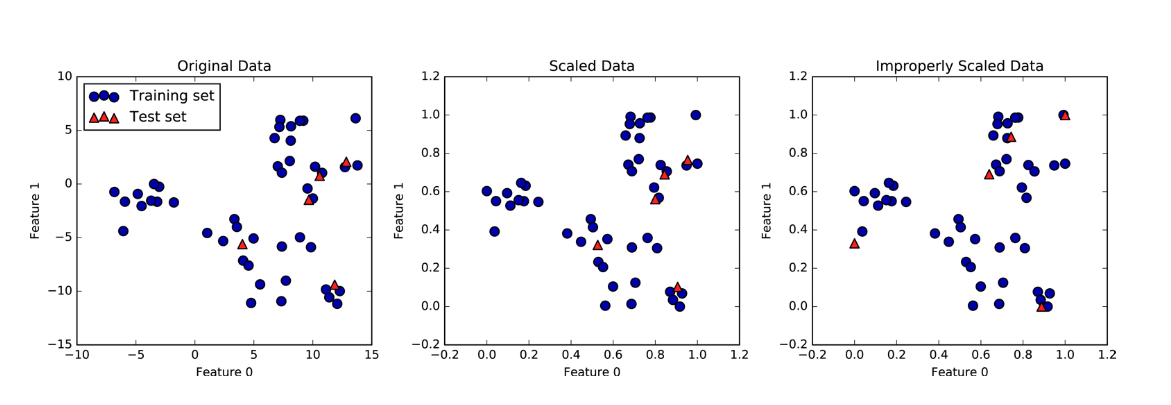
\includegraphics[width=13cm]{normalization-effect.png}
\end{figure}
The correct procedure is to normalize the training set and then once we have a stable model we can normalize also the test set with the same min and max values computed for the training set.

\section{NLP and Word Embedding}
Natural language processing is a field of deep learning in which you focus on recognizing elements of written text speech particles. Other fields of use are the summarization of text, question answering, automatic email response and forwarding, chatbots ecc ecc\\
Word embedding is a field of deep learning. It aims to represent a word as feature vectors, and consequently as numbers. The simplest way is to assign each word of a vocabulary a number but this way you could sort words which doesn't map as a semantic characterstic for words. A different way is to use a one-hot vector for each words. These vectors are the size of the vocabulary and only for the word we want to represent we put 0 in the corresponding position, otherwise 0. This representation has some pros: it's simple and it doesnt imply ordering. The cons: huge vectors and no embedded meaning.\\
The next idea is to represent words in a semantic space through vectors that can carry the essence of the meaning. We could, for example, place words on a real scale where the negative half expresses how negative the essence of the word is on the contrary the positive axis imply positivity.\\ We could expand this model to include two dimensions, they could for example represent how abstract or, inversely, concrete a word is. This kind of representation is defintely a step up and we have a low dimensionality representation for words and there is an embedded meaning from which to derive semantic distance or closeness.
\subsection*{Word embedding process}
We take a corpus (be it general purpose or specialized for a given context). The embedding algorithm will use a high feature space (around 300) to try and position the words of the corpus in such space. We then want to validate the goodness of the model by using it in NLP tasks.\\
\subsubsection*{Word2Vec algorithm}
Is a technique for builiding a rich semantic word embedding space (by google 2013). The key idea is to have similar embeddings for words that have similar meaning and context.It works by creating a fake task: given a specific word in the middle of a sentence (the input word), the network is going to tell us the probability for every word in our vocabulaty of being near-by the word we chose. The "near-by" amount is a parameter that we define, usually 5 before and 5 after the input word. \\
The resulting neural network is composed by input, one hidden and output layer. There is no activation function on the hidden layer neurons. The dimensionality of the hidden layer is equal do the dimensionality of the embeddin (example 300)

\section{Convolutional Neural Netowrks}
Convolutional neural networks are closely related and widely used in computer vision. Image classification in particular is a core task in computer vision. Single and multiple object localization on images and videos.
\section{Images}
There's a semantic gap between the human understanding and view of an image and the one of a machine. For a machine our image is just a tensor of values between [0, 255]; if the image is in colour then we have three times the data to specifiy che blue, green and red component. A challenge that quickly arises is any change of view point which makes it that all the pixel values chanage. Background clutter is another challenge in computer vision, it refers to the presence in the image of a background with little contrast with respect to the object. Illumination alters the value of the pixels and should also take into account. An attempt to solve image classification is the process of extracting fine edges in the image to find corners. Right now the best approach for computer vision is a data-driven approach:
\begin{itemize}
    \item collect a dataset of images and labels
    \item use machine learning algorithms to trian a classifirer
    \item evaluate the classifier on new images
\end{itemize}
\subsection{Convolution Neural Networks for Image Classification}
Suppose we have a 64x64x3 image and we want to say if it is a cat. We restructure the three matrices related to the colours a single vector of length 12288 elements and start working from that with a neural network we are alredy familiar wtih. The problem is that with slightly bigger images (1000x1000x3 = 3 Millions) there's a problem handling that many parameters. For this reason the community started using covolutions. Convolutions are performed by applying a filter through inner product over every possible sub-matrix in the input matrix. 
\begin{figure}[htbp]
    \centering
    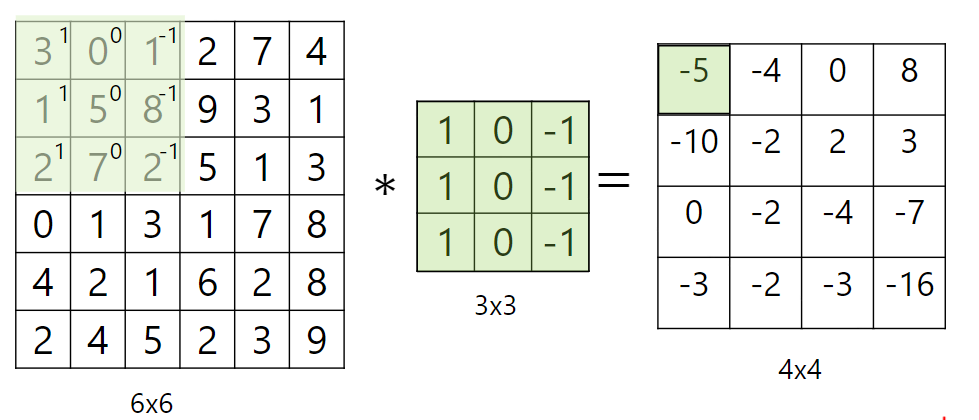
\includegraphics[width=12cm]{convolution_example.png}
\end{figure}
\begin{figure}[htbp]
    \centering
    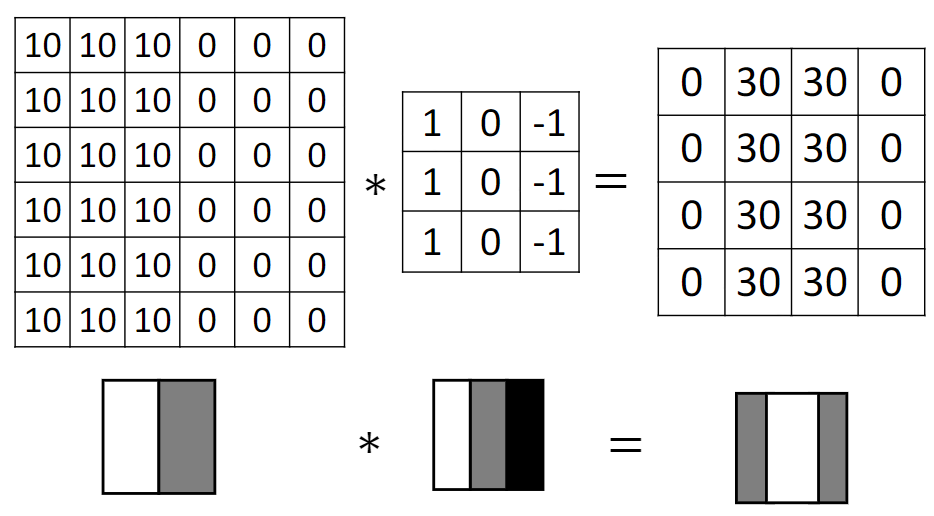
\includegraphics[width=12cm]{vertical_edge_example.png}
\end{figure}
Many handcrafted filters were created but right now, with Deep learning, we want to learn them. Since convolutions reduce the dimensionality of the matrix, if you want to preserve it you can add padding all around your matrix.\\
The amount of pixels by which you move your filter matrix over the input matrix is called stride, where a stride of 1 means moving pixel by pixel. A good balance between stride (speed) and accuracy must be found and it's dependant on the input images and the goal. For example, in big images the semantic meaning of neighbouring pixels is very similar and the information gained by having a strid of 1 is little so we might want to move faster.
\subsubsection{Convolutions on RGB images}
In the case of RGB images we have three filters or just a tensor of dimensionality 3. It is also possible to use two sets of filters to scout for different type of information from the original matrix. The matrix produced by the convolution is added with a bias for each convolutional matrix multiplication. The result of these operations is fed to an activation function ( often ReLU).
\subsubsection{Key Idea}
In traditional neural networks every input neuron is connected to all neurons of the next layer. In a convolutional layer we reshape the input tensor as a vector and each neuron of the second layer is going to be connected to the neurons involved in each image patch being filtered. The weights of the connection are going to be the values of the filter and are going to be learned. The weights used on every patch, which again are the filter values, are the same, this practice is called weight sharing. 
\subsubsection*{Back-propagation in CNN}
In CNN the backpropagation algorithm work as follow:
\begin{itemize}
    \item in the forward pass perform explicit computation with all the weights (some of them are the same)
    \item in the backward pass compure the gradient $\frac{\partial J}{\partial w_{1}}, \ldots,\frac{\partial J}{\partial w_{n}}$ for all the weights
    \item When updating the weights use the average of the gradients from the shared weights:
    \[ 
        w_1 = w_1-\alpha\left( \frac{\partial J}{\partial w_{1}}+\frac{\partial J}{\partial w_{4}}+\frac{\partial J}{\partial w_{7}}  \right)
    \]
\end{itemize}
Usually, on images with more than one channel filter weights are not shared among channels.\\
There are three types of layer used in a CNN:
\begin{itemize}
    \item Convolution layer
    \item Poolin layer
    \item Fully connected (standard) layer
\end{itemize}
\subsubsection*{Pooling layer: max pooling}
The pooling layer in a max-pooling operation moves around the image in patches just like the convolution layer but instead of applying a filter it extracts and outputs the max value of that patch.
\begin{figure}[htbp]
    \centering
    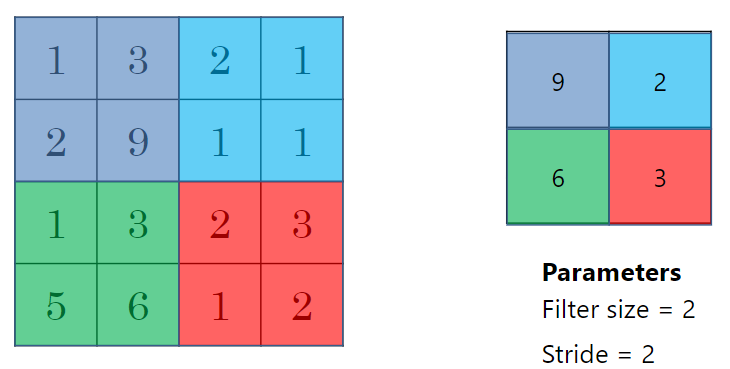
\includegraphics[width=10cm]{max_pooling.png}
\end{figure}
Other functions can be used in a pooling layer but empirical evidence shows that taking the max is the most effective operation.\\
Convolutions tend to reduce dimensionality of the input and it can happen that we loose details which causes a drop in accuracy.
\subsection{Visualizations - AlexNet Architecture}
AlexNet is one of the first successful applications of Deep Learning and convolutional neural networks. Its architecture uses a series of convolution in a phase called feature extraction and then after flattening the output of the convolutional part of the network, features are learned through a more traditional dense approach.\\
\subsubsection{Transfer Learning}
Suppose you have two datasets T and S: dataset S is fully annotated, very big and we can build a model $h_s$ for it. Dataset T instead is small but still annotated. We can use the model $h_s$ to learn a bettern $h_t$. This practice is called transfer learning. You can initialize the weight of the model for T to the value that the pre-trained model for S possess. This practice is most effective when S is bigger than the target T.\\ Of course the model for T will still need fine-tuning after the transfer of learning. To decide what and how many layers to fine-tune we can use this approach:
\begin{itemize}
    \item When T is very small with too few data, only fine-tune the dense layers
    \item When T is at least a little bit bigger try fine-tuning also the CNN layers but focus more on the last layers as the first ones capture low level feature and don't change much.
\end{itemize}
Alternatively you can use CNNs as a feature extractor to then feed into a traditonal or deep learning network. (Especially if T is very small)
\subsection{Modern ConvNets}
The VGG16 CNN presented by Oxford University is slightly deeper than AlexNet and uses only 3x3 filters because two 3x3 filters have a receptive field of one 5x5 filter. Deeper stacks of smaller filters are likely more powerful than a single larger filter:
\begin{itemize}
    \item You get more non-linearity for the same "size" of pattern learning
    \item There are less parameters
    \begin{itemize}
        \item A stack of three filters of 3x3(x3) = 27
        \item One larger 7x7 = 49
    \end{itemize}
\end{itemize}
\subsubsection{Residual Networks}
Using a Residual Network you can design very deep Neural Networks. Residual networks add shortcuts from earlier layers to layers that are further ahead in the architecture. A reason for adding these shortcuts is to use a layer to change the data drastically and focus on something very specific but at the same time we don't want to forget, loose track of the original data. If the dimensionality of the weight matrix don't match you can add an extra weight matrix to fix the issue. Reaserch has show that Residual Networks help prevent negative improvement as you train for more epochs.
\subsubsection*{1x1 Convolutions}
It can be useful to apply 1x1 convolutions on tensors that have many channels that you would like to reduce. Using multiple 1x1 convolutions on the same high channel number tensor we can reshape it to have the number of channels that we want. In doing multiple 1x1 convolutions we incorporate many non-linearity factors.
\subsubsection*{Inception Neural Network}
An idea that was proposed is to apply learning on filters of different sizes applied to tensors with many channels. The problem that resulted is that it was extremely computational costly. To solve this problem, before performing the 3x3 or 5x5 convolution they applied 1x1 convolutions to reduce the dimensionality. Operating like this relieved so much operational complexity. This set of convolutional passes are considered as a unit module and can be put together to form a chain of computation to increase the complexity of our model. It is also possible to introduce intermediate branches to calculate intermediate loss and 


\section{Optimization}
\subsection*{Batch-v.s.-Mini Batch Gradient Descent}
When using standard gradient descent you will use the entire test set to compute the cost function and the derivatives. Of course this is cost-prohibitive when the set is not very small. With mini-batch gradient descent you divide the test set into smaller batches and perform cost calculation and derivatives for each. Only after having run with every mini-batch you'll complete 1 epoch.\\
Stochastic gradient descent is a particular instance of batch gradient descent where batch size is 1. The speed of convergence for the three types can vary wildly and each comes with some tradeoff
\begin{figure}[htbp]
    \centering
    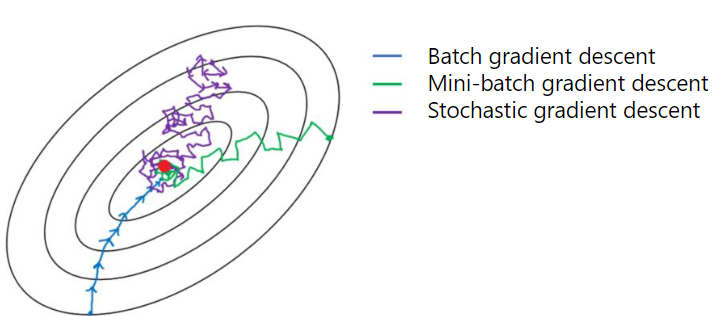
\includegraphics[width=10cm]{descent-comparison.png}
\end{figure}
Small train set size (about 2000 examples) is great for mini-batch. Batches are usually small powers of 2: 64, 128, 256, 512, 1024. Mini-batch size is also a learnable parameter and it's worth it to experiment with different values.

\subsection{Optimization Algorithms}
\subsubsection{Exponentially Weighted Average}
If your data plot is very noisy we can introduce some historic data about the observed variable and modify the current value taking a major component from the actual value but inserting a parametric component to smooth the curve.
\[ 
    V_t = \beta V_t+(1-\beta)\theta_t 
\]This way $V_t$ is the approximation of $\frac{1}{1-\beta}$ previous datapoint's value.
\begin{figure}[htbp]
    \centering
    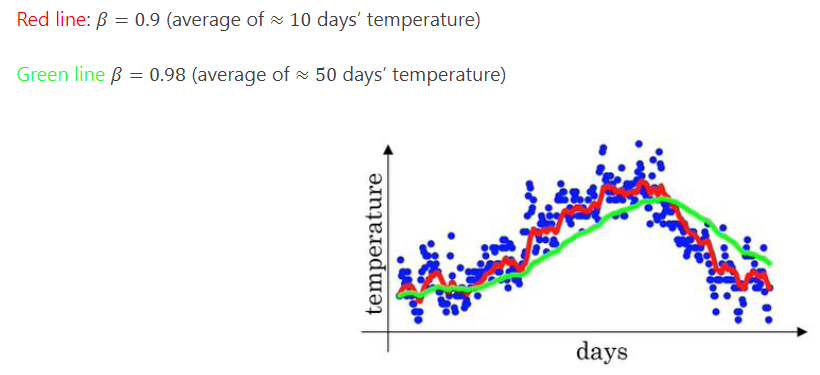
\includegraphics[width=10cm]{weighted_average.png}
\end{figure}
\subsubsection*{Bias Correction}
By implementing the formula $V_t = \beta V_t+(1-\beta)\theta_t $ with starting value $V_0 = 0$ the first few values are not correctly represented. We can then introduce the revised formula
\[ 
    \bar{V_t} = \frac{V_t}{1-\beta^t} 
\]By doing so, the added dividend will tend to 1, vanishing it's effect as $t \mapsto \infty$
\subsubsection*{Gradient Descent with Momentum}
In gradient descent with momentum we compute ad each iteration the derivatives $\frac{\partial L }{\partial w}, \frac{\partial L }{\partial b}$ and we compute:
\begin{align*}
    V_{dw}=\beta V_{dw}+(1-\beta)\frac{\partial L}{\partial w'} \quad V_{db}=\beta V_{db}+(1-\beta)\frac{\partial L}{\partial b'} \\
    W:= W - \alpha V_{dw'}\quad b:= b-\alpha V_{db}
\end{align*}
When considering Exponentially weighted averages in this case the average of b is more of less constant (vertical direction) while W goes towards the right. 
Gradient descent with momentum almost always works empirically  faster than standard gradient descent algorithm. 
\subsubsection*{RMSprop}
RMSprop is another improvement on gradient descent that relies on the idea of Exponentially weighted averages introducing a non-linearity by squaring the derivative value
\subsubsection*{ADAM}
ADAM or Adaptive Moment Estimation Optimizer is a optimization technique that puts together Grdient Descent with Momentum and RMSprop 

\subsubsection*{Learning Rate Decay}
Poorly choosing the value for your learning rate could prevent you from finding the minimum. A value too small could not converge or take too much time to do so. A value too large could end up jumping over your minimum and keep going back and forth. For this reason we implement learning rate decay and start with a larger value for the learning rate and gradually make it smaller to achieve better results.
\subsection*{Local Optimum in Neural Networks}
When observing the cost function it is very likely that it has saddle points and plateaus. Especially this last case is better handled by ADAM, RMSprop or Gradiant descent with momentum rather than the basic version.
\section{Loss Functions}
For binary classification we often use the binary cross-entropy loss where m is the number of examples in the mini-batch\\
For regression we often use the Mean Square error loss, again m is the number of examples in the mini-batch\\
For multiclass classification we usually insert a softmax activation function on the last layer of the network that will output a probability distribution over the classes. While the loss function used for multiclass classification is the Cross-Entropy loss. This function is used to evaluate the difference in two probability distribution (the one of the ground truth is given as a one-hot vector)
\section{Convolutional Neural Networks - Object Detection}
Image Classification can then be further categorized in the case that we want to localize the object placing it within its bounding box. When we are talking about multiple object localization we are talking about object detection. Our image classification network is modified as follows, adding a regression module/task for deciding the bounding box
\begin{figure}[htbp]
    \centering
    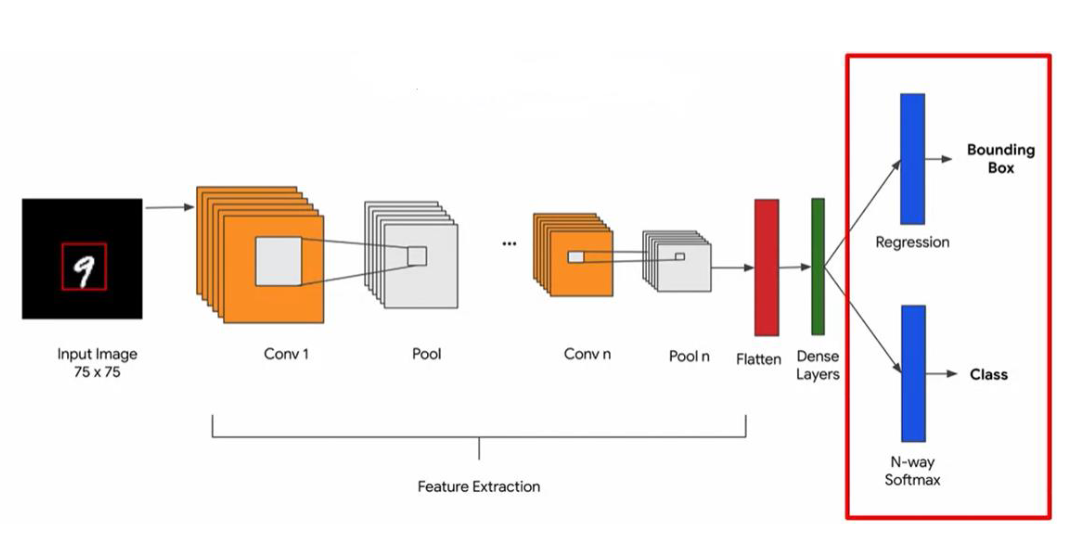
\includegraphics[width = 10cm]{object-localization-network.png}
\end{figure}
The output of the network will be a vector that has one binary digit to express whether the network thinks there is an object or not, followed by the four coordinates of the bounding box and then a one-hot subvector for the classification.
\subsection*{Landmark Detection}
Landmark detection is an application of object detection used to identify a fixed number of landmarks on an object to capture its detailed characterstics. It is often used on faces to capture emotions, pose estimation for animation etc. The ground truth for these landmark detection task is a vector with a binary for face or no face, for example, and then 64 coordinates (x,y) for each of the landmarks to be estimated.
\subsection*{Sliding Window detection}
A popular practice to perform object detection is to use a sliding window that moves through the image and each image patch is used as input for our trained Convolution NN. In order to handle different scales we can also change the size of the window.
\subsection*{Convolution implementation of sliding windows}
By removing the fully connected layers at the end of a CNN and replacing them with a series of 1x1 convolutions we have that the final value of a certain pixel in the last convolution result is only dependant on a specific window of pixel in the original image, hence obtaining a sliding window apprach withouth any other computation. 
\subsection*{Yolo Algorithm}
Yolo algorithm is a particular implementation of windowed object detection which uses a grid of $ n\times n $ squares, for example n=3. Then for every square it outputs a vector (of size let's say m) in the same form as a standard object detection (0/1 object or not, bounding box coordinates and one-hot subvector for class identified). The output is then going to be $n\times n\times m$. Using a convolutional implementation of sliding window the result tensor of the network is going to be based exclusively on the corresponding square in the grid.
\subsection*{Evaluating Object localization}
To evaluate the goodness of an object localization algorithm we can use a simple calculation of Intersection over Union that gives us a percentage of overlap. Then we apply a non-max suppression algorithm that works by removing all object detection that are scoring too poorly and then focusing on the best match. 

\section{Exercises}
\renewcommand{\arraystretch}{1.5}
\subsection*{Neural Network}
\subsubsection*{Exercise 1}
Consider the following neural network which takes two binary-valued inputs $x_1,x_2 \in {0,1}$ and outputs $h_\theta(x)$. Which of the following logical function does it compute?
\begin{figure}[htbp]
    \centering
    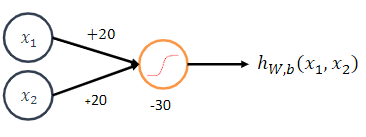
\includegraphics[width=10cm]{ExerciseBook/01-NeuralNetwork/exercise1.png}\newline
\end{figure}\newline
To anser we can simply compute the truth table for the possible values of $x_1, x_2$.
\begin{center}
    
    \begin{tabular}{ |c |c |c |}
        \hline
        \textbf{$x_1$} & \textbf{$x_2$} & \textbf{$h_{W,b}(x_1,x_2)$} \\
        \hline
        0 & 0 & -30 (0) \\ 
        0 & 1 & -10 (0) \\  
        1 & 0 & -10 (0) \\
        1 & 1 & 10 (1)\\
        \hline
    \end{tabular}
    Answer: logical AND
\end{center}
\subsubsection*{Exercise 2}
Consider the following neural network:
\begin{figure}[htbp]
    \centering
    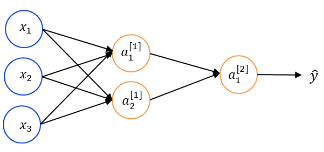
\includegraphics[width=10cm]{ExerciseBook/01-NeuralNetwork/exercise2.png}\newline
\end{figure}
I start by computing the activation vector $z^{[1]}$ by multiplying $W\cdot x+b^{[1]}$.
\[ 
    z^{[1]}=
    \begin{bmatrix}
        -1 \\
        8 
    \end{bmatrix}
\]
\\I then plug the activation vector into the activation function to get $a^{[1]} = g(z^{[1]}) = \frac{1}{1-e^{-z^{[1]}}}$
\[ 
    a^{[1]}=
    \begin{bmatrix}
        0.268941 \\
        0.999665
    \end{bmatrix}
\]\\I repeat for the next layer
\[ 
    z^{[2]}=
    \begin{bmatrix}
        2.537547
    \end{bmatrix}
\]
\\We conclude $a^{[2]}=0.926732$
\subsubsection*{Exercise 3}
\begin{figure}[htbp]
    \centering
    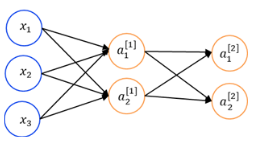
\includegraphics[width=10cm]{ExerciseBook/01-NeuralNetwork/exercise3.png}\newline
\end{figure}
I start by computing the activation vector $z^{[1]}$ by multiplying $W\cdot x+b^{[1]}$.
\[ 
    z^{[1]}=
    \begin{bmatrix}
        4 \\
        -16
    \end{bmatrix}
\]
\[ 
    a^{[1]}=
    \begin{bmatrix}
        0.982014 \\
        0.00000012 \\ 
    \end{bmatrix}
\]
\[ 
    z^{[2]}=
    \begin{bmatrix}
        2.964028 \\
        3.964027
    \end{bmatrix}
\]
\[ 
    a^{[2]}=
    \begin{bmatrix}
        0.268941 \\
        0.731058
    \end{bmatrix}
\]
\subsubsection*{Esercise 4}
In this diagram which we hand-drew in lecture, what do the horizontal axis (x-axis) and vertical axis (y-axis) represent?
\begin{figure}[htbp]
    \centering
    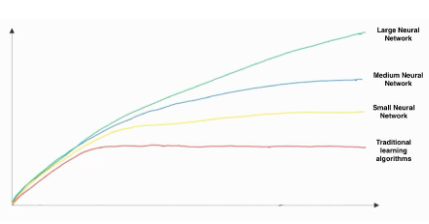
\includegraphics[width=10cm]{ExerciseBook/01-NeuralNetwork/exercise4.png}\newline
\end{figure}
Answer: x-axis is the amount of data; y-axis (vertical axis) is the performance of the algorithm.
\subsubsection*{Exercise 5}
Which one of these plots represents a ReLU activation function?
\begin{figure}[htbp]
    \centering
    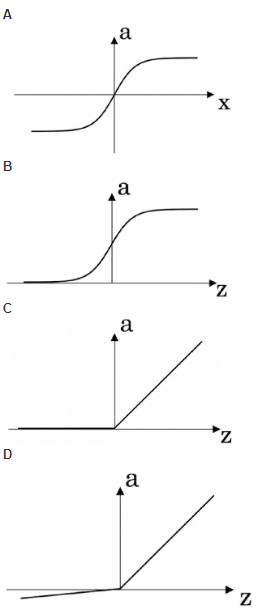
\includegraphics[width=6cm]{ExerciseBook/01-NeuralNetwork/exercise5.png}\newline
\end{figure}
Solution answer C
\subsubsection*{Exercise 6}
Which of these is the "Logistic Loss"?\\
Solution answer A
\subsubsection*{Exercise 7}
Consider the following computation graph. What is the output J?
\begin{figure}[htbp]
    \centering
    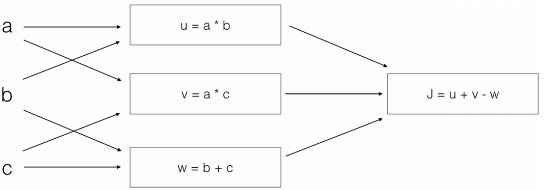
\includegraphics[width=12cm]{ExerciseBook/01-NeuralNetwork/exercise7.png}\newline
\end{figure}
Solution answer B
\subsubsection*{Exercise 8}
You are building a binary visual classifier for recognizing apples(y=1) vs. tomatoes(y=0). Which one of these activation functions would yourecommend using for the output layer?
\\Solution: answer C : Sigmoid because it's perfect for linear classification between [0,1]
\subsubsection*{Exercise 9}
Suppose you have built a neural network. You decide to initialize the weights and biases to be zero. Which of the following statements is true?\\
Solution answer A: Each neuron in the first hidden layer will perform the same computation. So even after multiple iterations of gradient descent each neuron in the layer will becomputing the samething as other neurons.
\subsubsection*{Exercise 10}
Consider the following 2 hidden layer neural network, which of the following statements are True?
\begin{figure}[htbp]
    \centering
    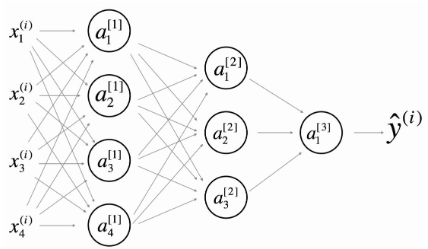
\includegraphics[width=12cm]{ExerciseBook/01-NeuralNetwork/exercise10.png}\newline
\end{figure}
Solution, answers A, B, F
\subsubsection*{Exercise 11}
The dev and test set should:
Solution answer A: come from the same distribution.
\subsubsection*{Exercise 12}
If your Neural Network model seems to underfit your data, what of the following would be promising things to try?\\
Solution answers: B, C
\end{document}
